% ###################################
%      Chromatic Amplitude Detuning
\section{\review{Chromatic Amplitude Detuning}}

The Chromatic Amplitude Detuning is the tune shift dependant on both the actions and the momentum
offset, whose decapole contributed terms are described via a Taylor expansion in
\cref{eq:decapoles:chromatic_ampdet:decapole_contribution}. More information and derivations can
be found in \cref{subsection:detuning_effects:chromatic_amplitude_detuning} and
\cref{appendix:chromatic_amplitude_detuning}.

\begin{equation}
  \begin{aligned}
    \Delta Q(J_x, J_y, \delta) = 
    & \frac{\partial^2Q}{\partial J_x \partial \delta}    \cdot J_x\delta 
    + \frac{\partial^2 Q}{\partial J_y \partial \delta}   \cdot J_y\delta 
    + \frac{1}{3!} \frac{\partial^3 Q}{\partial \delta^3} \cdot \delta^3.
    \end{aligned}
    \label{eq:decapoles:chromatic_ampdet:decapole_contribution}
\end{equation}


The last term is more commonly referred to as the third order chromaticity, $Q'''$.  Each of those
terms depend on the $\beta$-functions, the horizontal dispersion $D$ and the normalized decapole
field gradient $K_5$ for a single source of length $L$,

\begin{equation}\begin{aligned}
  \frac{\partial^2 Q_x}{\partial J_x \partial \delta} =& \frac{1}{16 \pi} K_5L \beta_x^2 D,         &\quad
  \frac{\partial^2 Q_x}{\partial J_y \partial \delta} =& -\frac{1}{8\pi} K_5L \beta_x \beta_y D,
\\
  \frac{\partial^3 Q_x}{\partial \delta^3}            =& \frac{1}{4\pi} K_5L \beta_x D^3,           &\quad
  \frac{\partial^2 Q_y}{\partial J_x \partial \delta} =& -\frac{1}{8\pi} K_5L \beta_x \beta_y D,
\\
  \frac{\partial^2 Q_y}{\partial J_y \partial \delta} =& \frac{1}{16 \pi} K_5L \beta_y^2 D,        &\quad 
  \frac{\partial^3 Q_y}{\partial \delta^3}            =& -\frac{1}{4\pi} K_5L \beta_y D^3.
\end{aligned}\end{equation}

The action dependant terms can be measured by exciting the beam with an AC-dipole with increasing
strengths at different momentum-offsets.

Such a measurement was taken with octupole and decapole correctors turned off to measure the bare
machine. Some data could not be collected due to machine availability issues, restricting the
measurement to low intensity kicks. 
Nevertheless, the terms $\frac{\partial^2 Q_x}{\partial J_y \partial \delta}$ and $\frac{\partial^2
Q_y}{\partial J_y \partial \delta}$ for beam 2 were measured for the first time in the LHC. The
momentum-offsets measured at were $-0.001$ and $0.001$, respectively roughly equal to a trim of 
$+140$Hz and $-140$Hz of the RF.

\Cref{figure:decapoles:chromatic_amplitude_detuning:b2qxy}
and~\cref{figure:decapoles:chromatic_amplitude_detuning:b2qyy} show a fit of those terms to measured
$Q_{x,y}$ vs $J_{y}$ at two different momentum offsets. Expected shifts from MADX-PTC simulations,
that include field errors ranging from sextupoles to decahexapoles ($b_3$ to $b_8$ and $a_4$ to
$a_8$) are shown as a comparison.

% Studies and plots in 
% jupyter/chromatic_amplitude_detuning/simulations/2022-10-19_vs_PTC/Analytical_Chromatic_Detuning.ipynb

\begin{figure}[H]
  \centering
  \begin{subfigure}{0.8\textwidth}
      \centering
      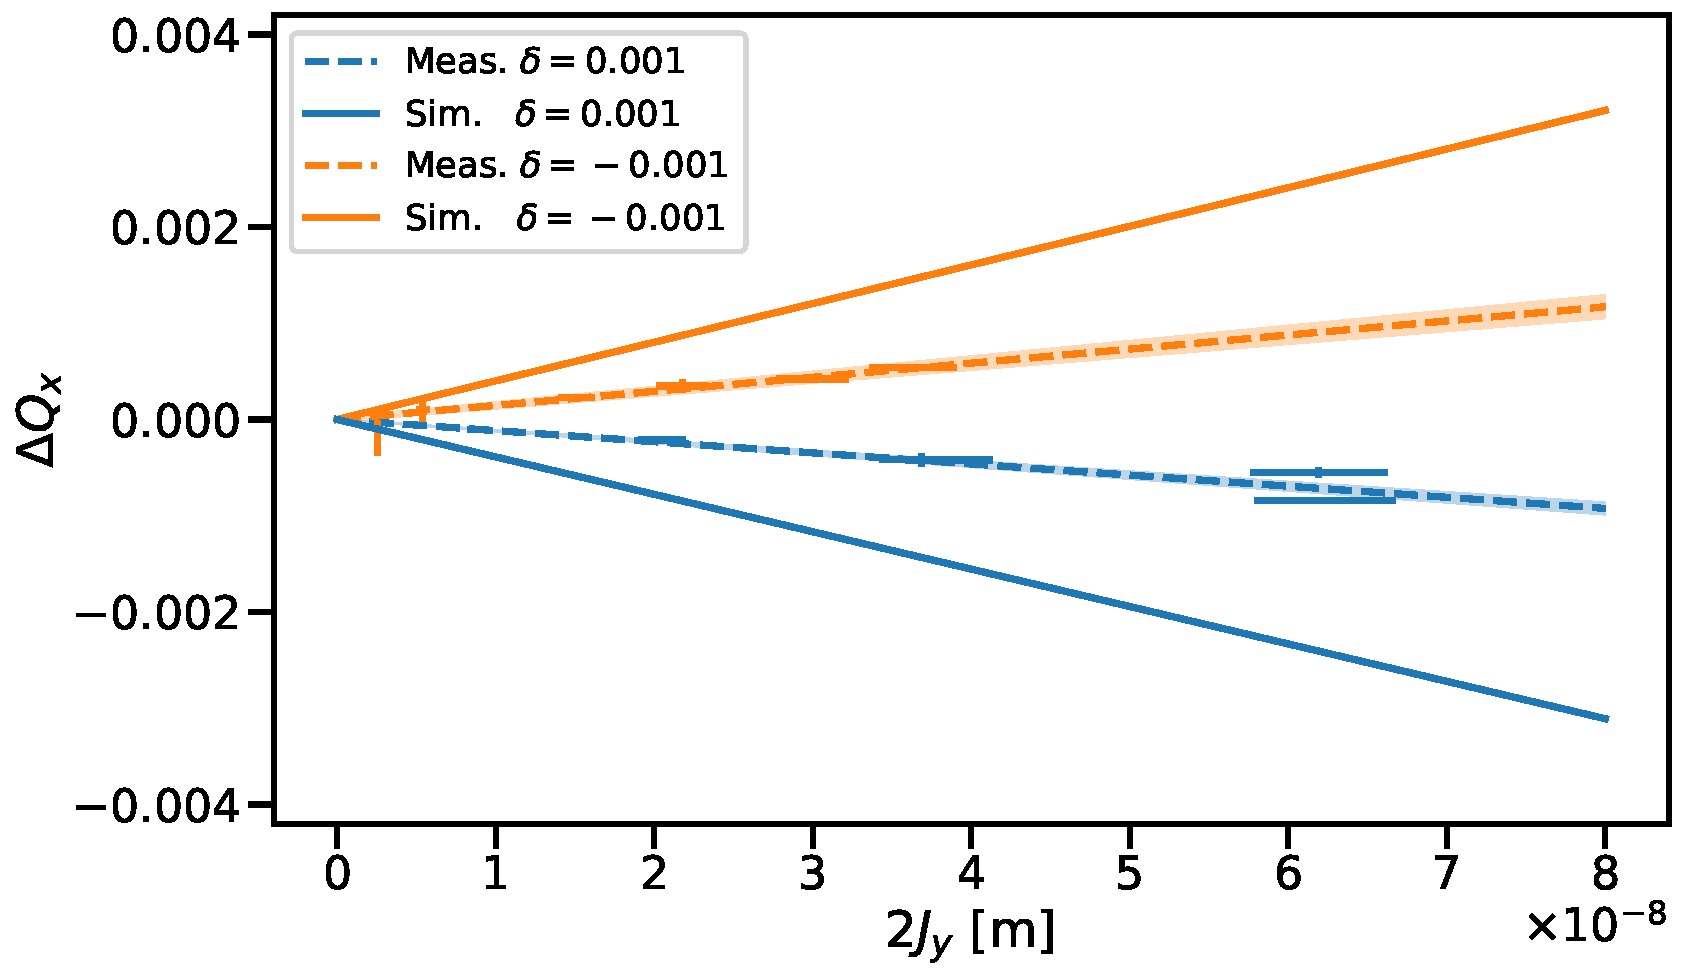
\includegraphics[width=\textwidth]{images/chromatic_amplitude_detuning/B2_Qxy_decay0.00.pdf}
      \caption{Horizontal tune shift depending on the vertical action: 
      $\frac{\partial^2 Q_x}{\partial J_y \partial \delta}$.}
      \label{figure:decapoles:chromatic_amplitude_detuning:b2qxy}
  \end{subfigure}
  %
  \\[1em]
  %
  \begin{subfigure}{0.8\textwidth}
      \centering
      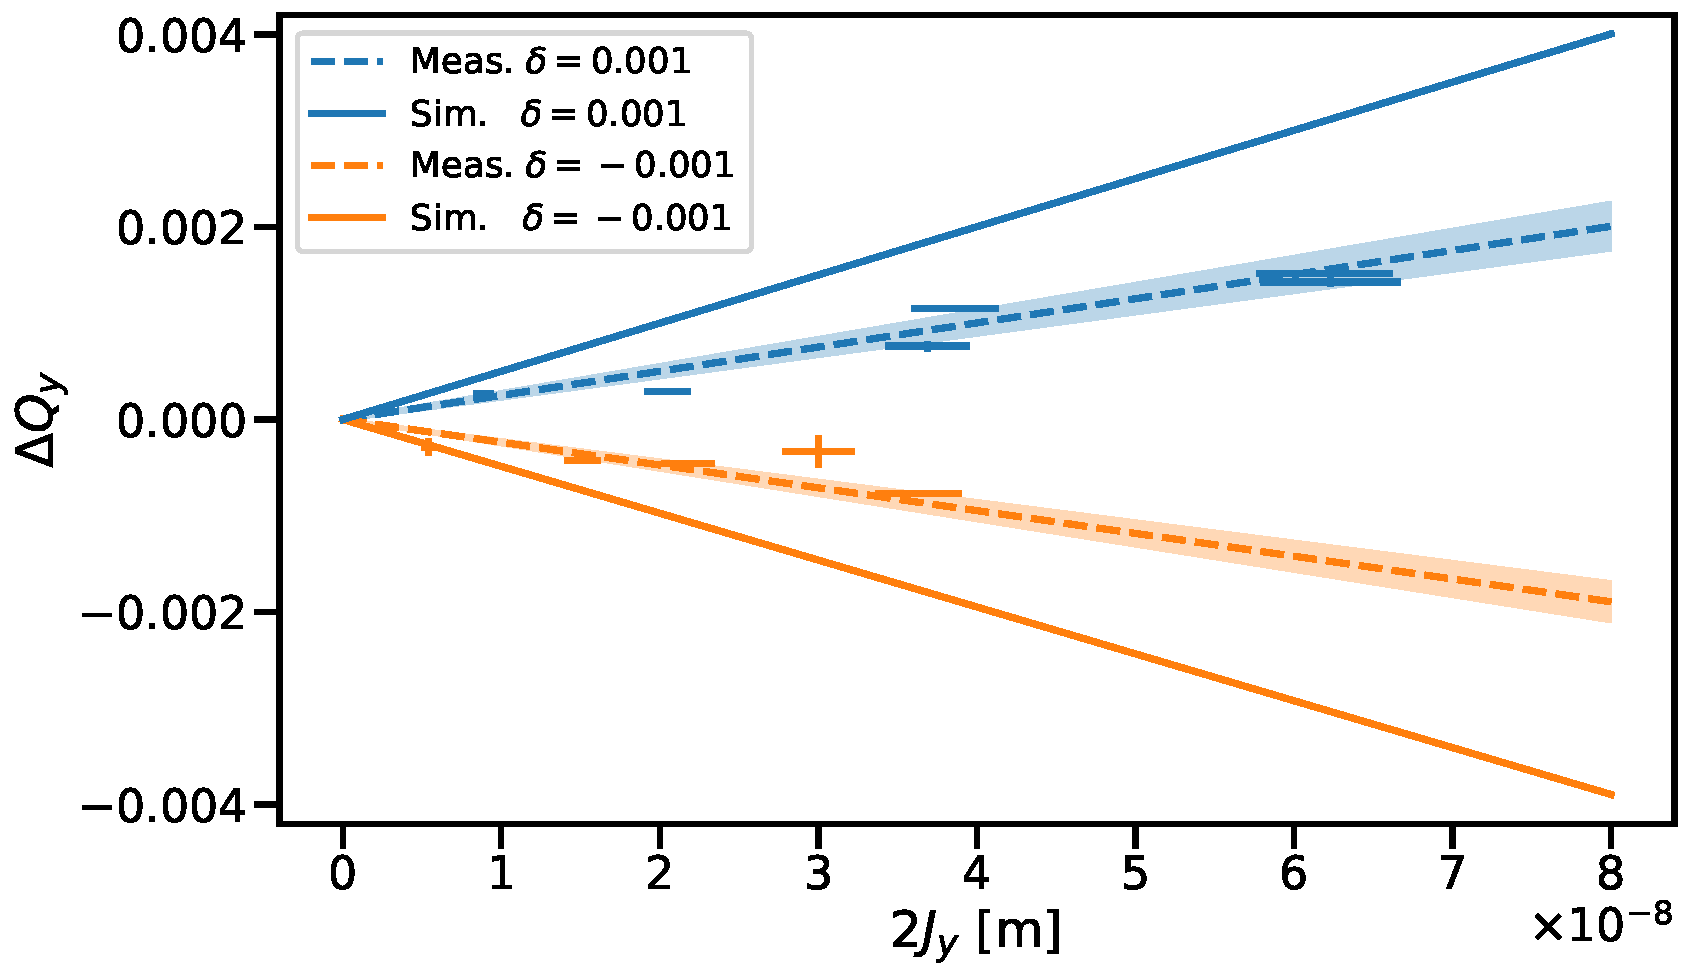
\includegraphics[width=\textwidth]{images/chromatic_amplitude_detuning/B2_Qyy_decay0.00.pdf}
      \caption{Vertical tune shift depending on the vertical action: 
      $\frac{\partial^2 Q_y}{\partial J_y \partial \delta}$.}
      \label{figure:decapoles:chromatic_amplitude_detuning:b2qyy}
  \end{subfigure}
  \caption{Measured and simulated tune shift due to a change of action via an AC-Dipole at two
  different momentum offsets. Each fit corresponds to a chromatic amplitude detuning term evaluated
  at a certain $\delta$.}
  \label{figure:decapoles:chromatic_amplitude_detuning:two_terms}
\end{figure}


\begin{table}[H]
  \centering
  \begin{tabular}{lrr}
  \toprule
   Type  & $\frac{\partial^2 Q_x}{\partial J_y \partial \delta}[10^{4}\mathrm{m}^{-1}]$ & $\frac{\partial^2 Q_y}{\partial J_y \partial \delta}[10^{4}\mathrm{m}^{-1}]$ \\
  \midrule
  $\delta = +0.001$ & & \\
  \hspace{2mm}Meas.  &   -1.16 ± 0.08 &   1.26 ± 0.15 \\
  \hspace{2mm}Sim.   &   -3.82 ± 0.01 &   2.47 ± 0.01 \\
  \hspace{2mm}Ratio  &    0.30 ± 0.02 &   0.51 ± 0.06 \\
  $\delta = -0.001$ & & \\
  \hspace{2mm}Meas.  &  1.47 ± 0.12  &  -1.18 ± 0.13 \\
  \hspace{2mm}Sim.   &  3.92 ± 0.01  &  -2.41 ± 0.01 \\
  \hspace{2mm}Ratio  &  0.38 ± 0.03  &   0.49 ± 0.05 \\
  \bottomrule
  \end{tabular}
  \caption{Comparison of the measured and simulated terms $\frac{\partial^2 Q_x}{\partial J_y
   \delta}$ and $\frac{\partial^2 Q_y}{\partial J_y \partial \delta}$ via PTC, at two
  discrete momentum offsets. Simulations include errors from normal sextupole to decahexapole and
  from skew octupole to decahexapole.}
  \label{table:decapoles:chromatic_ampdet}
\end{table}



A consistent difference between simulation and measurement is observed, which values and
ratios of measurement to model can be found in \cref{table:decapoles:chromatic_ampdet}.
The observed ratios of measurement to model for the chromatic amplitude detuning show slight
discrepancies compared to the bare chromaticity ones. These discrepancies could be due to the low
intensity kicks, which don't allow for a better fit. However, the similarity of the ratios suggests
an issue with the decapolar error model of the main dipoles, with measurements showing values about
half of those predicted by the magnetic model.